\documentclass[a4paper]{article}

\usepackage[utf8]{inputenc}
\usepackage[T1]{fontenc}
\usepackage{graphicx}
\usepackage[frenchb]{babel}
\usepackage{amsmath}
\usepackage{listings}

% define our color
\usepackage{xcolor}

% code color
\definecolor{ligthyellow}{RGB}{250,247,220}
\definecolor{darkblue}{RGB}{5,10,85}
\definecolor{ligthblue}{RGB}{1,147,128}
\definecolor{darkgreen}{RGB}{8,120,51}
\definecolor{darkred}{RGB}{160,0,0}

% other color
\definecolor{ivi}{RGB}{141,107,185}


\lstset{
    language=scilab,
    captionpos=b,
    extendedchars=true,
    frame=lines,
    numbers=left,
    numberstyle=\tiny,
    numbersep=5pt,
    keepspaces=true,
    breaklines=true,
    showspaces=false,
    showstringspaces=false,
    breakatwhitespace=false,
    stepnumber=1,
    showtabs=false,
    tabsize=3,
    basicstyle=\small\ttfamily,
    backgroundcolor=\color{ligthyellow},
    keywordstyle=\color{ligthblue},
    morekeywords={include, printf, uchar},
    identifierstyle=\color{darkblue},
    commentstyle=\color{darkgreen},
    stringstyle=\color{darkred},
}

\begin{document}

\title{VISA -- TP3 : Stéréovision dense}
\author{Arnaud Cojez}
\date{mardi 4 octobre 2016}

\maketitle

\newpage
\tableofcontents
\newpage
%----------------------------------------------------------------------------------------
%	INTRODUCTION
%----------------------------------------------------------------------------------------

\section{Introduction}

\subsection{Motivation}
Lors du dernier TP sur la mise en correspondance stéréoscopique, nous avons utilisé une méthode de stéréoscopie dite "éparse". Celle-ci consistait en l'utilisation d'une sélection de points pour la mise en correspondance entre 2 images. Ce qui nous permettait de retrouver des informations de profondeur grâce à 2 projections de la même scène, avec des points de vues différents.\\

Nous allons ici mettre en œuvre une méthode de mise en correspondance stéréoscopique dense. C'est-à-dire que nous allons utiliser tous les pixels d'une projection, et non une sélection de points, afin de calculer la disparité entre l'image gauche et l'image droite.

\subsection{La stéréovision dense}
Le but de cette méthode est de créer une carte de disparité entre chaque pixel de deux projections. La disparité correspond à la différence d'abscisse entre deux points considérés comme homologues pour les deux images.\\

Pour simplifier les calculs, nous allons utiliser une configuration de stéréoscope canonique. C'est une configuration dans laquelle :
\begin{itemize}
\item les deux caméras sont identiques ;
\item les axes optiques sont parallèles ;
\item les deux capteurs d’image sont coplanaires ;
\item les lignes horizontales des capteurs sont confondues.\\
\end{itemize}

Cette configuration possède plusieurs avantage qui nous soulagent de certaines étapes d'estimations ou de réctifications (ex. réctification épipolaire). C'est pour cette raison que nous allons utiliser une méthode de stéréovision dense, avec des images issues d'un stéréoscope canonique.\\

Nous allons utiliser cette méthode sur ces deux images en niveau de gris.
\begin{figure}[h]
\begin{center}
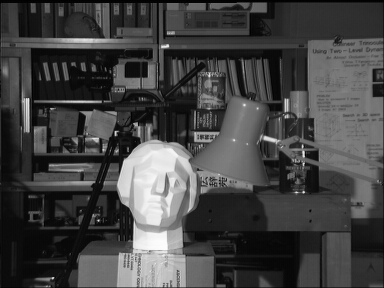
\includegraphics[width=170px]{left.png}
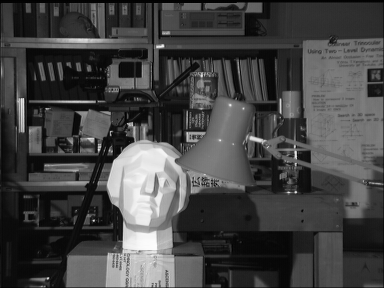
\includegraphics[width=170px]{right.png}
\end{center}
\caption{Image gauche et Image droite}
\end{figure}

\clearpage
%--------------------------------------------------------------------------
%	SIMILARITÉ PAR SSD
%--------------------------------------------------------------------------

\section{Calcul de l'image de disparité gauche}
Pour calculer l'image de disparité relative aux points de l'image de gauche, nous devons suivre plusieurs étapes.

\subsection{Image intermédiaire mMinSSD}
Cette étape consiste à calculer l'image intermédiaire minSSD. Cette matrice est de la même taille que l'image de gauche donnée en paramètre.
Chaque élément de cette matrice se verra assigner la valeur $dMinSSD = (2 * iWindowHalfSize + 12 * iWindowHalfSize + 1)^2 * 512.0$, qui correspond au maximum possible de SSD (sum of squared differences).

\begin{lstlisting}
// ---------------------------------------------------------
/// \brief Estime la disparite par minimisation du SSD, image gauchee
/// prise comme reference.
///
/// @param psLeftImage: image gauche
/// @param psRightImage: image droite
/// @param iMaxDisparity: disparite maximale recherchee
/// @param iWindowHalfSize: demi-taille de la fenetre de correlation
/// @return carte des disparites calculee
// ---------------------------------------------------------
Mat iviLeftDisparityMap(const Mat& mLeftGray,
                      const Mat& mRightGray,
                      int iMaxDisparity,
                      int iWindowHalfSize) {
  [...]

  Mat mMinSSD(mLeftGray.size(), CV_64F);

  [...]

  // Initialisation de l'image du minimum de SSD
  dMinSSD = pow((double)(2 * iWindowHalfSize + 1), 2.0) * 512.0;
  for (iRow = iWindowHalfSize;
      iRow < mMinSSD.size().height - iWindowHalfSize;
      iRow++) {
      // Pointeur sur le debut de la ligne
      pdPtr1 = mMinSSD.ptr<double>(iRow);
      // Sauter la demi fenetre non utilisee
      pdPtr1 += iWindowHalfSize;
      // Remplir le reste de la ligne
      for (iCol = iWindowHalfSize;
          iCol < mMinSSD.size().width - iWindowHalfSize;
          iCol++)
              *pdPtr1++ = dMinSSD;
  }

  [...]
}
\end{lstlisting}

Nous avons donc les valeurs de SSD maximales dans cette matrice, valeurs que nous tenterons de réduire dans la partie suivante, en cherchant la SSD minimale pour chaque point.

\clearpage
\subsection{Image intermédiaire mSSD}
Maintenant que nous avons cette base des SSD maximum, nous pouvons calculer les vraies SSD, qui seront stockées temporairement dans la matrice mSSD.
Le but est de calculer la SSD minimale de chaque point en se servant des pixels de la même ligne. Le résultat obtenu sera stocké dans la matrice mSSD. Si le résultat est inférieur à la SSD minimale (contenue dans mMinSSD), alors celui-ci viendra remplacer l'ancienne valeur dans mMinSSD.

La SSD est calculée dans iviComputeLeftSSDCost, méthode que nous implémenterons dans la sous-partie suivante.

\begin{lstlisting}
/// [...]
Mat iviLeftDisparityMap(const Mat& mLeftGray,
                        const Mat& mRightGray,
                        int iMaxDisparity,
                        int iWindowHalfSize) {
  [...]
  Mat mSSD(mLeftGray.size(), CV_64F);
  [...]
    // Boucler pour tous les decalages possibles
    for (iShift = 0; iShift < iMaxDisparity; iShift++) {
        // Calculer le cout SSD pour ce decalage
        mSSD = iviComputeLeftSSDCost(mLeftGray, mRightGray,
                                     iShift, iWindowHalfSize);
        // Mettre a jour les valeurs minimales
        for (iRow = iWindowHalfSize;
            iRow < mMinSSD.size().height - iWindowHalfSize;
            iRow++) {
            // Pointeurs vers les debuts des lignes
            pdPtr1 = mMinSSD.ptr<double>(iRow);
            pdPtr2 = mSSD.ptr<double>(iRow);
            pucDisparity = mLeftDisparityMap.ptr<unsigned char>(iRow);
            // Sauter la demi fenetre non utilisee
            pdPtr1 += iWindowHalfSize;
            pdPtr2 += iWindowHalfSize;
            pucDisparity += iWindowHalfSize;
            // Comparer sur le reste de la ligne
            for (iCol = iWindowHalfSize;
                iCol < mMinSSD.size().width - iWindowHalfSize;
                iCol++) {
                // SSD plus faible que le minimum precedent
                if (*pdPtr1 > *pdPtr2) {
                    *pucDisparity = (unsigned char)iShift;
                    *pdPtr1 = *pdPtr2;
                }
                // Pixels suivants
                pdPtr1++; pdPtr2++; pucDisparity++;
            }
        }
    }
}
\end{lstlisting}

\subsection{Calcul de la SSD pour l'image gauche}

\subsubsection{Explications}
Pour calculer une SSD pour l'image de gauche, nous allons utiliser cette formule, trouvée dans le cours :
\begin{equation}
\sum_{i=-w_x}^{w_x} \sum_{i=-w_y}^{w_y} (I_l(x_l+i,y+j)-I_r(x_l+i-s,y+j))^2
\end{equation}

\subsubsection{Implémentation C++}
\begin{lstlisting}
// ---------------------------------------------------------
/// \brief Calcule la somme des differences aux carre, image gauche
/// prise comme reference.
///
/// @param psLeftImage: image gauche
/// @param psRightImage: image droite
/// @param iShift: decalage teste
/// @param iWindowHalfSize: demi-taille de la fenetre de correlation
/// @return somme des differences au carre pour chaque x,y
// ---------------------------------------------------------
Mat iviComputeLeftSSDCost(const Mat& mLeftGray,
                          const Mat& mRightGray,
                          int iShift,
                          int iWindowHalfSize) {
    Mat mLeftSSDCost(mLeftGray.size(), CV_64F);

    for(int x = 0; x < mLeftGray.cols - iWindowHalfSize; x++) {
      for(int y = 0; y < mLeftGray.rows - iWindowHalfSize; y++) {
        double diff_sum = 0.;

        for(int i = -iWindowHalfSize; i < iWindowHalfSize; i++) {
          for(int j = -iWindowHalfSize; j < iWindowHalfSize; j++) {
            double diff = ((double) mLeftGray.at<unsigned char>(y + j, x + i) - (double) mRightGray.at<unsigned char>(y + j, x + i - iShift));
            diff_sum += pow(diff, 2.);
          }
        }
        mLeftSSDCost.at<double>(y, x) = diff_sum;

      }
    }
    return mLeftSSDCost;
}
\end{lstlisting}

\subsubsection{Résultats}

L'éxecution du programme nous donne comme résultat l'image de disparité suivante (ré-échantillonnée pour des raisons de visibilité) :
\begin{figure}[h]
\begin{center}
	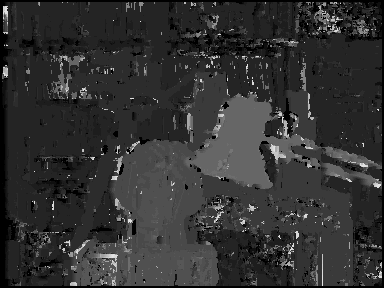
\includegraphics[width=200px]{left-disparity_resampled.png}
\end{center}
\caption{Carte de disparité gauche -- ré-échantillonnée}
\end{figure}
Nous retrouvons certaines formes présentes dans l'image source, telles que la lampe et le visage. Pour faire une analyse plus poussée, nous allons générer une carte de disparités similaires, mais cette fois-ci pour l'image de droite.

\clearpage
%----------------------------------------------------------------------------------------
%	VÉRIFICATION GAUCHE-DROITE
%----------------------------------------------------------------------------------------

\section{Vérification gauche-droite}
Nous avons besoin des cartes de disparité des 2 images pour reconstituer l'information de profondeur. Nous allons donc reproduire la même procédure, mais cette fois-ci pour l'image de droite.

\subsection{Calcul de la SSD pour l'image droite}

\subsubsection{Explications}
Nous allons reprendre les mêmes calculs, à quelques subtilitées près : on échange les matrices droites et gauche, et on additionne le décalage s au lieu de le soustraire.
\begin{equation}
\sum_{i=-w_x}^{w_x} \sum_{i=-w_y}^{w_y} (I_r(x_r+i,y+j)-I_l(x_r+i+s,y+j))^2
\end{equation}

\subsubsection{Implémentation C++}

\begin{lstlisting}
// ---------------------------------------------------------
/// \brief Estime la disparite par minimisation du SSD, image droite
/// prise comme reference.
///
/// @param psLeftImage: image gauche
/// @param psRightImage: image droite
/// @param iMaxDisparity: disparite maximale recherchee
/// @param iWindowHalfSize: demi-taille de la fenetre de correlation
/// @return carte des disparites calculee
// ---------------------------------------------------------
Mat iviRightDisparityMap(const Mat& mLeftGray,
                         const Mat& mRightGray,
                         int iMaxDisparity,
                         int iWindowHalfSize) {
Mat mSSD(mRightGray.size(), CV_64F);
Mat mMinSSD(mRightGray.size(), CV_64F);
Mat mRightDisparityMap(mRightGray.size(), CV_8U);// Images pour les resultats intermediaires
double dMinSSD, *pdPtr1, *pdPtr2;
unsigned char *pucDisparity;
int iShift, iRow, iCol;

    // Initialisation de l'image du minimum de SSD
    dMinSSD = pow((double)(2 * iWindowHalfSize + 1), 2.0) * 512.0;
    for (iRow = iWindowHalfSize;
        iRow < mMinSSD.size().height - iWindowHalfSize;
        iRow++) {
        // Pointeur sur le debut de la ligne
        pdPtr1 = mMinSSD.ptr<double>(iRow);
        // Sauter la demi fenetre non utilisee
        pdPtr1 += iWindowHalfSize;
        // Remplir le reste de la ligne
        for (iCol = iWindowHalfSize;
            iCol < mMinSSD.size().width - iWindowHalfSize;
            iCol++)
                *pdPtr1++ = dMinSSD;
    }
    // Boucler pour tous les decalages possibles
    for (iShift = 0; iShift < iMaxDisparity; iShift++) {
        // Calculer le cout SSD pour ce decalage
        mSSD = iviComputeRightSSDCost(mLeftGray, mRightGray,
                                     iShift, iWindowHalfSize);
        // Mettre a jour les valeurs minimales
        for (iRow = iWindowHalfSize;
            iRow < mMinSSD.size().height - iWindowHalfSize;
            iRow++) {
            // Pointeurs vers les debuts des lignes
            pdPtr1 = mMinSSD.ptr<double>(iRow);
            pdPtr2 = mSSD.ptr<double>(iRow);
            pucDisparity = mRightDisparityMap.ptr<unsigned char>(iRow);
            // Sauter la demi fenetre non utilisee
            pdPtr1 += iWindowHalfSize;
            pdPtr2 += iWindowHalfSize;
            pucDisparity += iWindowHalfSize;
            // Comparer sur le reste de la ligne
            for (iCol = iWindowHalfSize;
                iCol < mMinSSD.size().width - iWindowHalfSize;
                iCol++) {
                // SSD plus faible que le minimum precedent
                if (*pdPtr1 > *pdPtr2) {
                    *pucDisparity = (unsigned char)iShift;
                    *pdPtr1 = *pdPtr2;
                }
                // Pixels suivants
                pdPtr1++; pdPtr2++; pucDisparity++;
            }
        }
    }
    return mRightDisparityMap;
}
\end{lstlisting}
\clearpage
\begin{lstlisting}
// ---------------------------------------------------------
/// \brief Calcule la somme des differences aux carre, image droite
/// prise comme reference.
///
/// @param psLeftImage: image gauche
/// @param psRightImage: image droite
/// @param iShift: decalage teste
/// @param iWindowHalfSize: demi-taille de la fenetre de correlation
/// @return somme des differences au carre (double 64bits)
// ---------------------------------------------------------
Mat iviComputeRightSSDCost(const Mat& mLeftGray,
                           const Mat& mRightGray,
                           int iShift,
                           int iWindowHalfSize) {
    Mat mRightSSDCost(mLeftGray.size(), CV_64F);

    for(int x = 0; x < mRightGray.cols - iWindowHalfSize; x++) {
      for(int y = 0; y < mRightGray.rows - iWindowHalfSize; y++) {
        double diff_sum = 0.;

        for(int i = -iWindowHalfSize; i < iWindowHalfSize; i++) {
          for(int j = -iWindowHalfSize; j < iWindowHalfSize; j++) {
            double diff = ((double) mRightGray.at<unsigned char>(y + j, x + i) - (double) mLeftGray.at<unsigned char>(y + j, x + i + iShift));
            diff_sum += pow(diff, 2.);
          }
        }
        mRightSSDCost.at<double>(y, x) = diff_sum;

      }
    }
    return mRightSSDCost;
}
\end{lstlisting}
\clearpage
\subsubsection{Résultats}
Nous obtenons ici une image similaire à la carte de disparité gauche. En observant attentivement, nous pouvons remarquer que la lampe, entre autres, se trouve plus à gauche que dans l'image précédente. Cela est dû à la profondeur de la scène. La lampe est située plus près de la caméra, donc elle sera plus décalée quand le point de vue aura changé.

\begin{figure}[h]
\begin{center}
	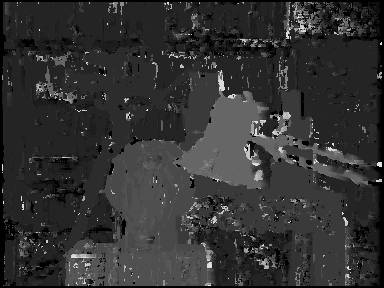
\includegraphics[width=200px]{right-disparity_resampled.png}
\end{center}
\caption{Carte de disparité droite -- ré-échantillonnée}
\end{figure}

Maintenant que nous disposons des deux cartes de disparités, nous allons pouvoir les mettre en commun pour en tirer certaines estimations.

\clearpage
%----------------------------------------------------------------------------------------
%	COHÉRENCE GAUCHE-DROITE
%----------------------------------------------------------------------------------------
\section{Cohérence gauche-droite}

\subsection{Explications}
Nous disposons désormais des cartes de disparités gauches et droites. Grâce à elles nous allons créer une carte de cohérence entre l'image de gauche et l'image de droite. Cette carte nous permettra de repérer les paires de pixels non homologues.\\
Nous en profiterons par conséquent pour créer un masque de validité, constitué de pixels noirs à l'emplacement des pixels homologues, et d'un pixel blanc quand aucune paire n'a été formée.\\

Pour ce faire, nous allons parcourir les pixels de l'image de gauche, et faire des vérifications sur la cohérence des coordonnées des pixels, en vérifiant ces formules :
\begin{equation}
  d_r(x,y) = d_l(x+d_r(x,y),y)
\end{equation}
\begin{equation}
  d_l(x,y) = d_r(x-d_l(x,y),y)
\end{equation}

Par conséquent, deux actions sont possibles :
\begin{itemize}
\item Lorsque ces deux formules se réalisent pour un pixel donné :
  \begin{enumerate}
    \item on copie le pixel correspondant de l'image de gauche (image de référence) dans la carte de disparité ;
    \item on ajoute un pixel noir dans la carte de validation ;
  \end{enumerate}
\item dans le cas contraire :
  \begin{enumerate}
    \item on copie le pixel correspondant de l'image de gauche (image de référence) dans la carte de disparité ;
    \item on ajoute un pixel noir dans la carte de validation.
  \end{enumerate}
\end{itemize}

\clearpage
\subsection{Implémentation C++}

\begin{lstlisting}
// ---------------------------------------------------------
/// \brief Verifie la coherence des cartes gauche et droite.
///
/// @param psLeftDisparity: carte gauche des disparites
/// @param psRightDisparity: carte droite des disparites
/// @param psValidityMask: carte des disparites valides
/// @return carte des disparites fusionnee
// ---------------------------------------------------------
Mat iviLeftRightConsistency(const Mat& mLeftDisparity,
                            const Mat& mRightDisparity,
                            Mat& mValidityMask) {

    Mat mDisparity(mLeftDisparity.size(), CV_8U);

    for(int x = 0; x < mLeftDisparity.cols; x++) {
      for (int y = 0; y < mLeftDisparity.rows; y++) {
        double dl = (double) mLeftDisparity.at<unsigned char>(y, x);
        double dr = (double) mRightDisparity.at<unsigned char>(y, x);

        double dlStep = (double) mLeftDisparity.at<unsigned char>(y, x + dr);
        double drStep = (double) mRightDisparity.at<unsigned char>(y, x - dl);

        if(dl == drStep && dr == dlStep) {
          mValidityMask.at<unsigned char>(y, x) = 0;
          mDisparity.at<unsigned char>(y, x) = (double) mLeftDisparity.at<unsigned char>(y, x);
        } else {
          mValidityMask.at<unsigned char>(y, x) = 255;
          mDisparity.at<unsigned char>(y,x) = 0;
        }
      }
    }
    return mDisparity;
}
\end{lstlisting}

\subsection{Résultats}

Nous avons comme résultat la carte de validité suivante, on distingue la plupart des contours des objets. Cela est dû au fait que certains points sur l'extérieur des objets sont occultés par le changement de point de vue. Réciproquement, le centre des objets est généralement teinté de noir car on y retrouve facilement des points homologues.

\begin{figure}[h]
\begin{center}
	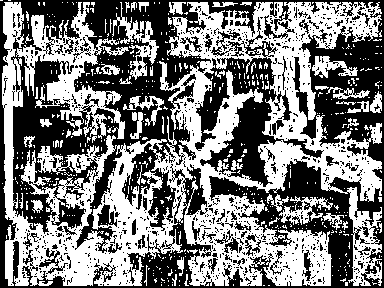
\includegraphics[width=200px]{validity-mask.png}
\end{center}
\caption{Carte de validité}
\end{figure}

Nous retrouvons à peu près les mêmes informations dans la carte de disparité gauche-droite. Mais nous pouvons également retrouver une information importante. En effet, on distingue différentes nuances de gris. La lambe possède un gris plus clair que la tête, qui possède un gris plus clair que la biliothèque, etc.
Nous pourrons par conséquent récupérer des informations sur la profondeur des objets dans la scène, par rapport au capteur.

\begin{figure}[h]
\begin{center}
	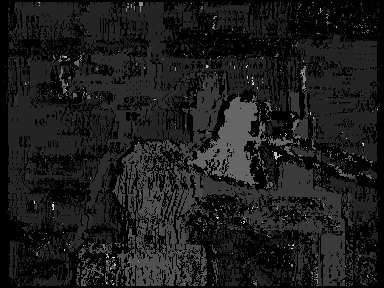
\includegraphics[width=200px]{disparity_resampled.png}
\end{center}
\caption{Carte de disparité -- ré-échantillonnée}
\end{figure}

\clearpage
%----------------------------------------------------------------------------------------

%----------------------------------------------------------------------------------------
%	CONCLUSION
%----------------------------------------------------------------------------------------

\section{Conclusion}
Pour pallier à la perte d'information de profondeur, nous avons mis en œuvre plusieurs méthode de stéréovision. Cette fois-ci, nous avons choisi d'utiliser une méthode de stéréovision dense.\\
Nous nous sommes dotés d'un stéréoscope canonique afin de nous épargner les étapes de rectifications épipolaires.\\

Contrairement à la méthode de stéréovision éparse vue dans le précédent TP, cette méthode prend en compte l'ensemble des pixels d'une image, par conséquent, les estimations de profondeurs sont plus précises. Cependant, les bords ainsi que les objets à l'arrière de la scène peuvent être occultés, résultant d'une absence d'informations dans ces zones.\\

Après application de cette méthode, nous avons pu extraire différentes cartes, exprimant des informations différentes, en particulier sur la situation des objets par rapport au capteur, dans une scène 3D. \\
Nous avons donc constaté qu'il existe différentes méthodes de stéréovision, avec leurs avantages et inconvénients.

\clearpage
%----------------------------------------------------------------------------------------

\section{Annexe}

\begin{figure}[h]
\begin{center}
	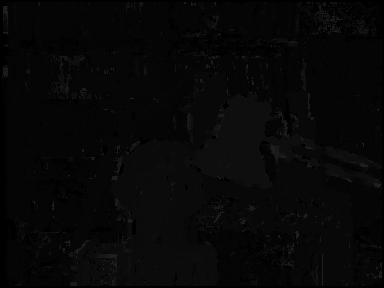
\includegraphics{left-disparity.png}
\end{center}
\caption{Carte de disparité gauche}
\end{figure}

\begin{figure}[h]
\begin{center}
	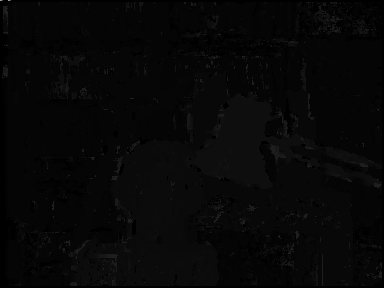
\includegraphics{right-disparity.png}
\end{center}
\caption{Carte de disparité droite}
\end{figure}

\begin{figure}[h]
\begin{center}
	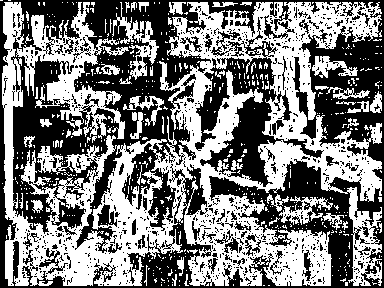
\includegraphics{validity-mask.png}
\end{center}
\caption{Carte de validité}
\end{figure}

\begin{figure}[h]
\begin{center}
	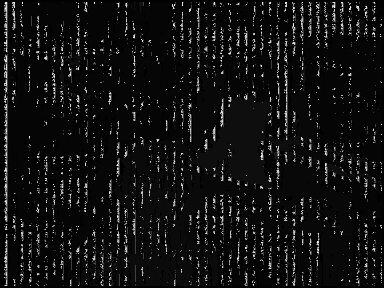
\includegraphics{disparity.png}
\end{center}
\caption{Carte de disparité}
\end{figure}

\end{document}
